\subsection{Вычислительные эксперименты}
    Возьмём параметры для модели:
    \[
        \begin{split}
            & \varepsilon_1 = 10, \varepsilon_2 = 8, \varepsilon_3 = 6, \\
            & \alpha_{12} = 6, \alpha_{13} = 2, \alpha_{23} = 0.5, \\
            & k_{12} = 4, k_{13} = 1, k_{23} = 0.5.
        \end{split}
    \]
    
    Тогда точки равновесия и их собственные значения равны:
    \[
        \begin{split}
            & x^{(0)} = (0,0,0), ~ \lambda_i = (10, 8, -6), \\
            & x^{(1)} = (0,24,16), ~ \lambda_i = (-166, ~ \pm i \cdot 6.93\dots), \\
            & x^{(2)} = (3,0,5), ~ \lambda_i = (77.5, ~ \pm i \cdot 7.74\dots), \\
            & x^{(3)} = (-3.458\dots, 46.66\dots, -150), ~ \lambda_i = (-160\dots, 153.5\dots, 6.54\dots), \\
        \end{split}
    \]

    При этом точка равновесия \( x^{(3)} \) не будет иметь влияния, поскольку находится на большом удалении в отрицательных координатах.

    \subsubsection{При вымершей первой популяции}

    \begin{figure}[H]
        \centering
        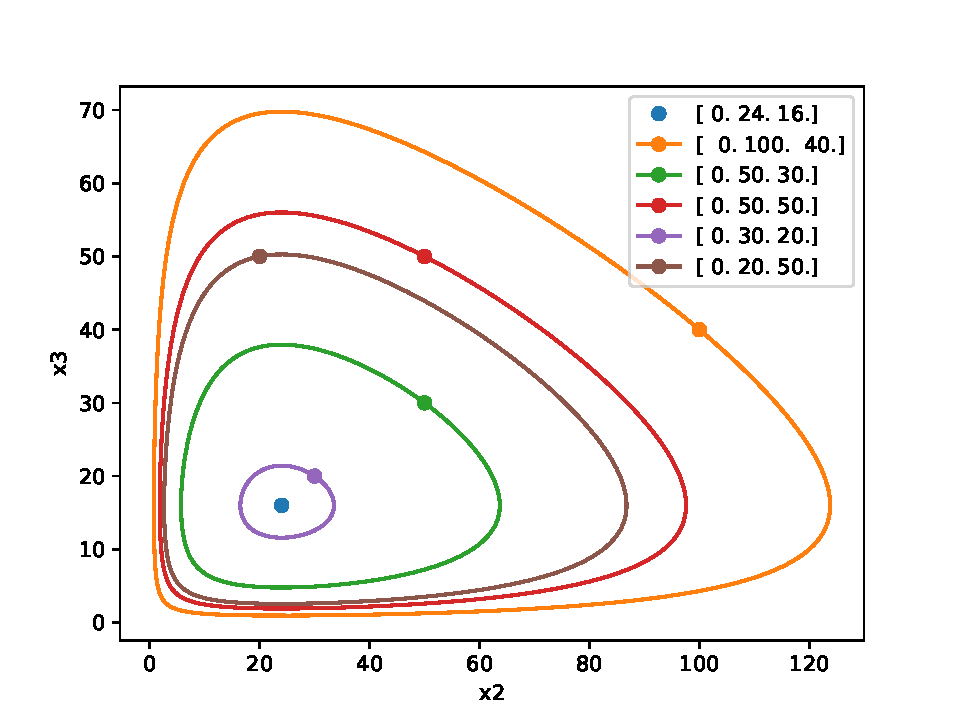
\includegraphics[width=8cm]{pictures/x1_0phase.pdf}
        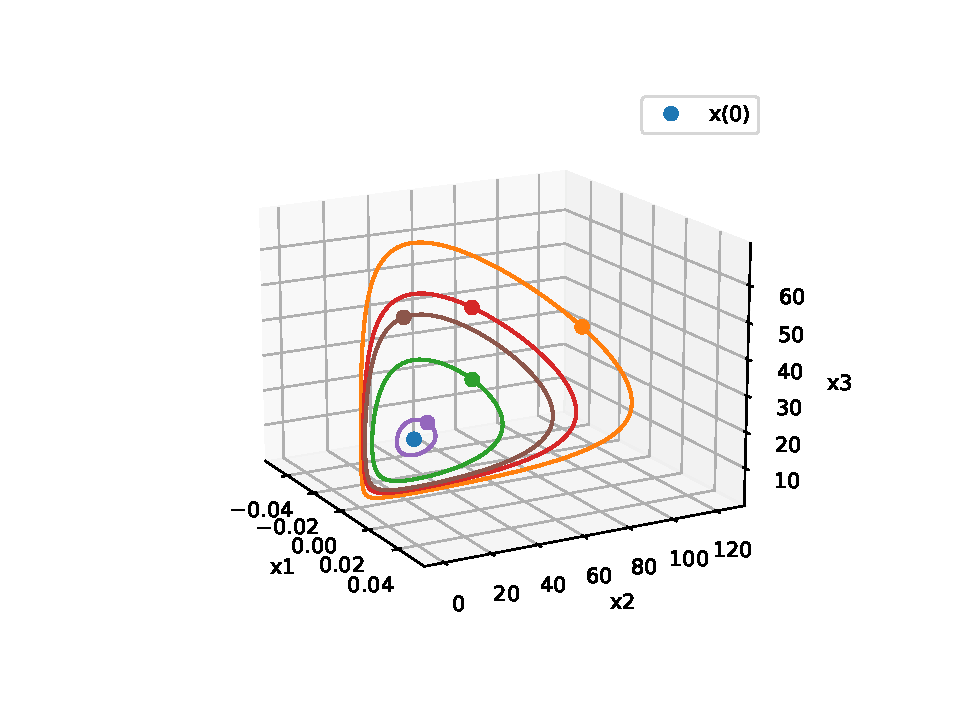
\includegraphics[width=8cm]{pictures/x1_0phase3.pdf}
        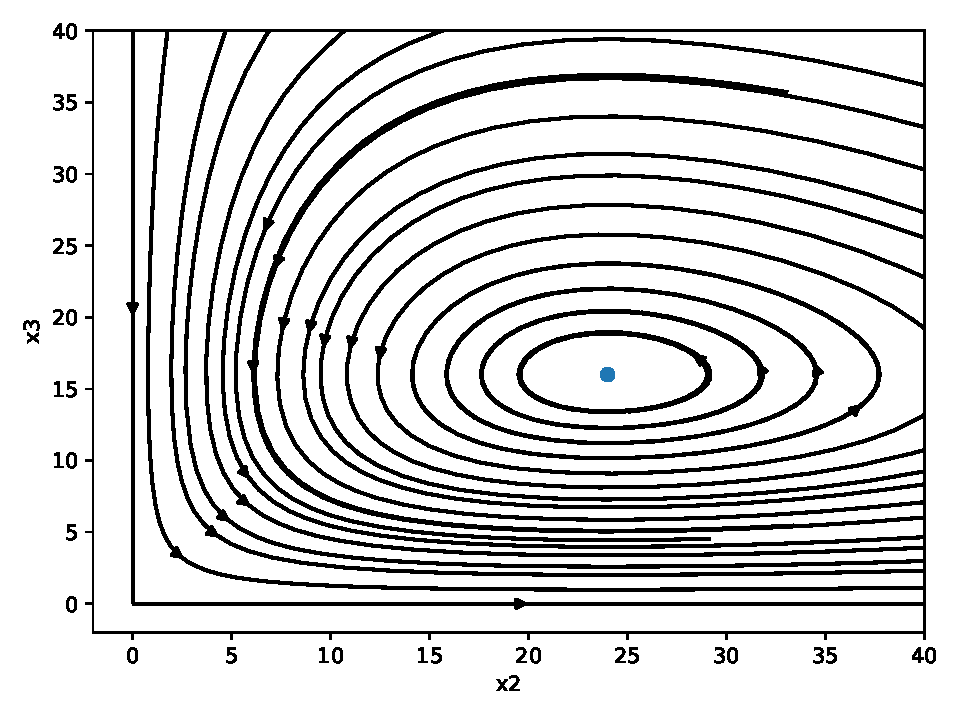
\includegraphics[width=8cm]{pictures/x1_0vector.pdf}
        \caption{На отрезке времени \( [0, 3] \).}\label{lvx1_0}
    \end{figure}
    При \(x_1 = 0\) (Рис. \ref{lvx1_0}) обе популяции хищников никогда не вымрут и будут двигаться по замкнутым кривым.


    \subsubsection{При вымершей второй популяции}

    \begin{figure}[H]
        \centering
        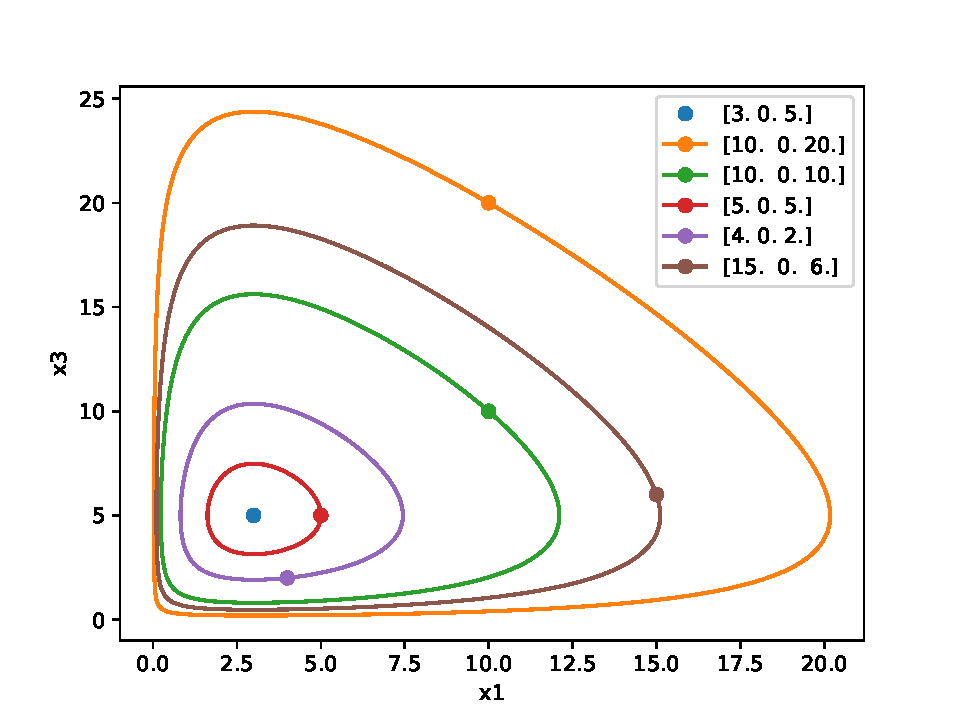
\includegraphics[width=8cm]{pictures/x2_0phase.pdf}
        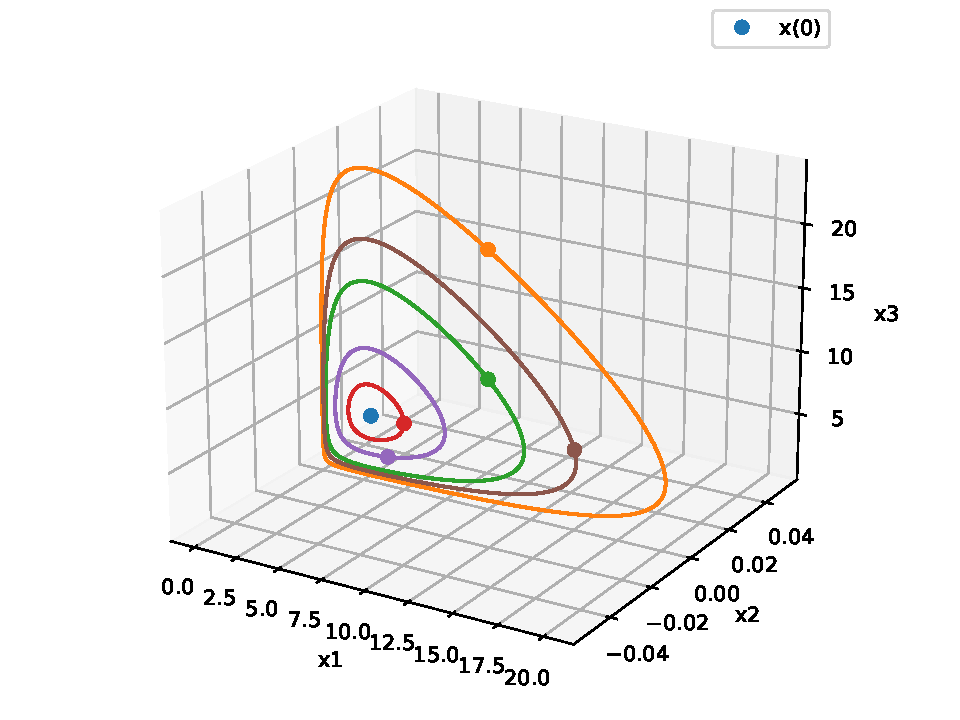
\includegraphics[width=8cm]{pictures/x2_0phase3.pdf}
        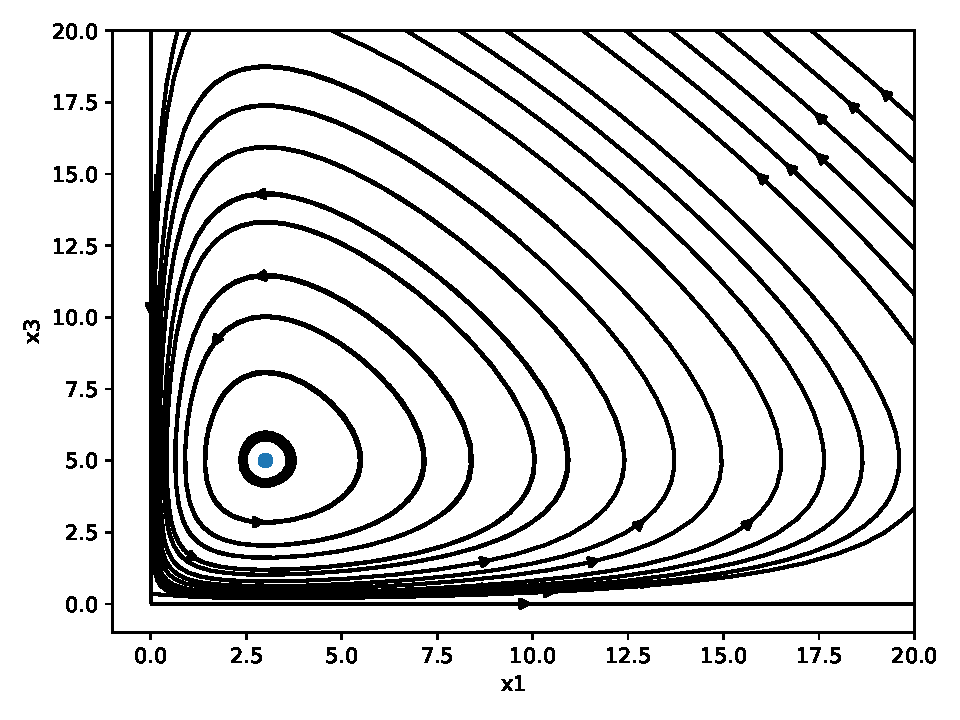
\includegraphics[width=8cm]{pictures/x2_0vector.pdf}
        \caption{На отрезке времени \( [0, 3] \).}\label{lvx2_0}
    \end{figure}
    При \(x_2 = 0\) (Рис. \ref{lvx2_0}) популяция жертв и вторая популяция хищников не вымрут и тоже будут двигаться по замкнутым кривым.


    \subsubsection{При вымершей третьей популяции}

    \begin{figure}[H]
        \centering
        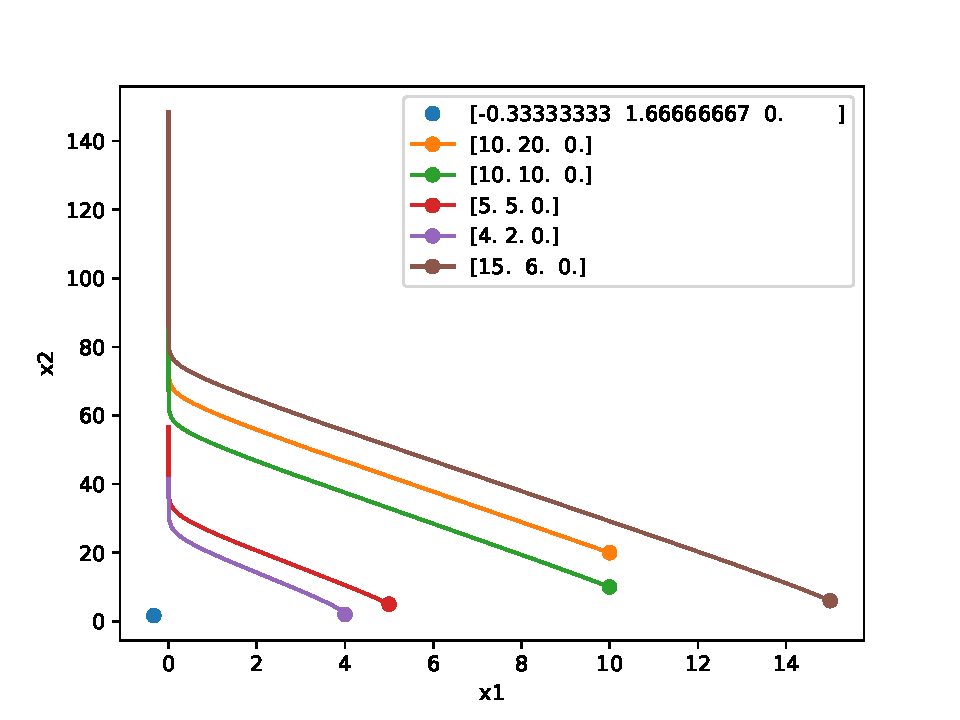
\includegraphics[width=8cm]{pictures/x3_0phase.pdf}
        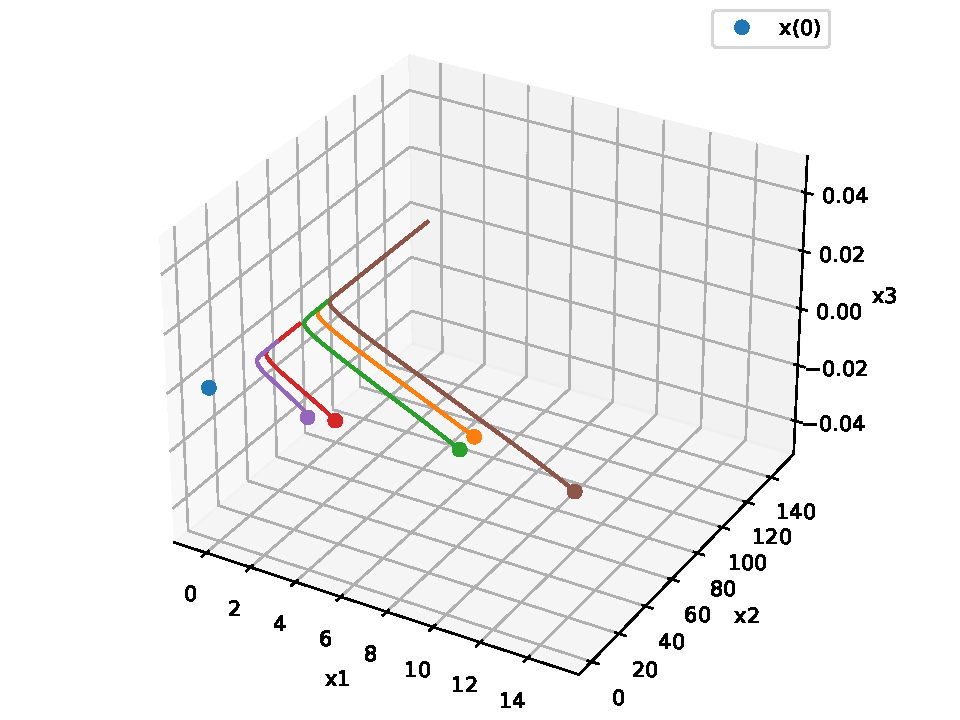
\includegraphics[width=8cm]{pictures/x3_0phase3.pdf}
        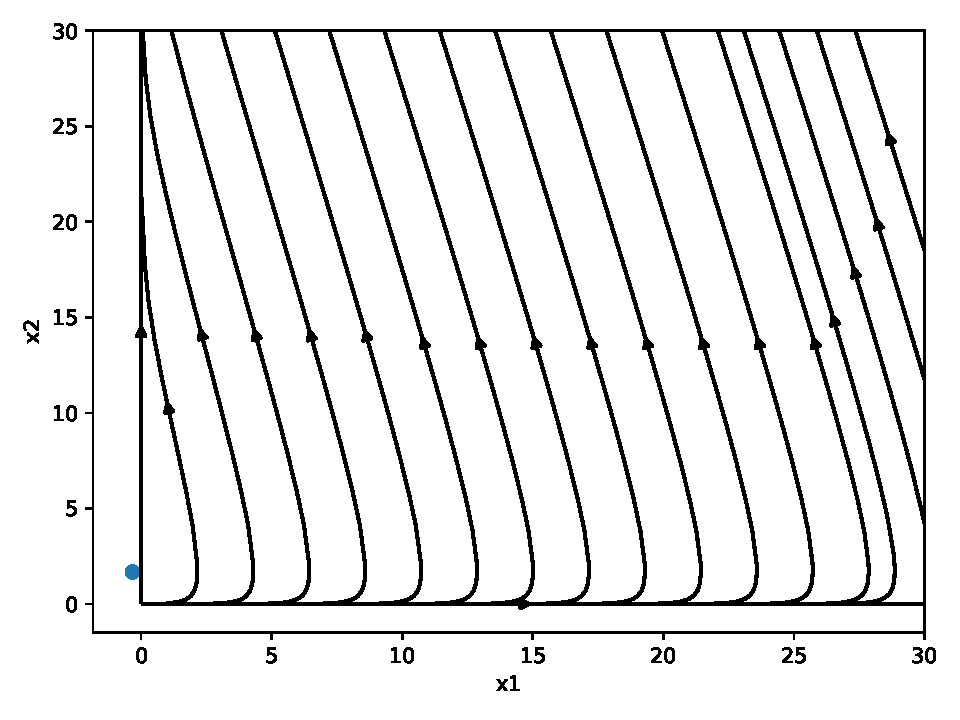
\includegraphics[width=8cm]{pictures/x3_0vector.pdf}
        \caption{На отрезке времени \( [0, 0.1] \).} \label{lvx3_0}
    \end{figure}
    При \(x_3 = 0\) (Рис. \ref{lvx3_0}) нулевая точка является неустойчивым узлом, при этом популяция жертв со временем вымрет, а первая популяция хищников безгранично будет увеличиваться.

    \subsubsection{Несколько изначально не вымерших популяций}
    Рассмотрим поведение решений во всей исследуемой области.
    \begin{figure}[H]
        \centering
        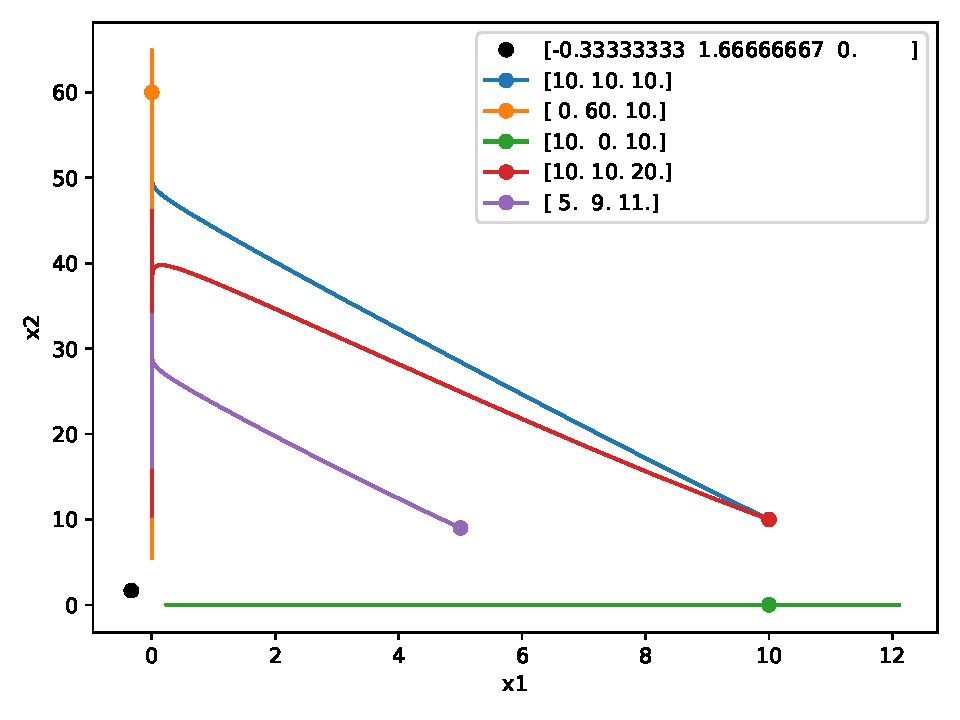
\includegraphics[width=8cm]{pictures/x_12phase.pdf}
        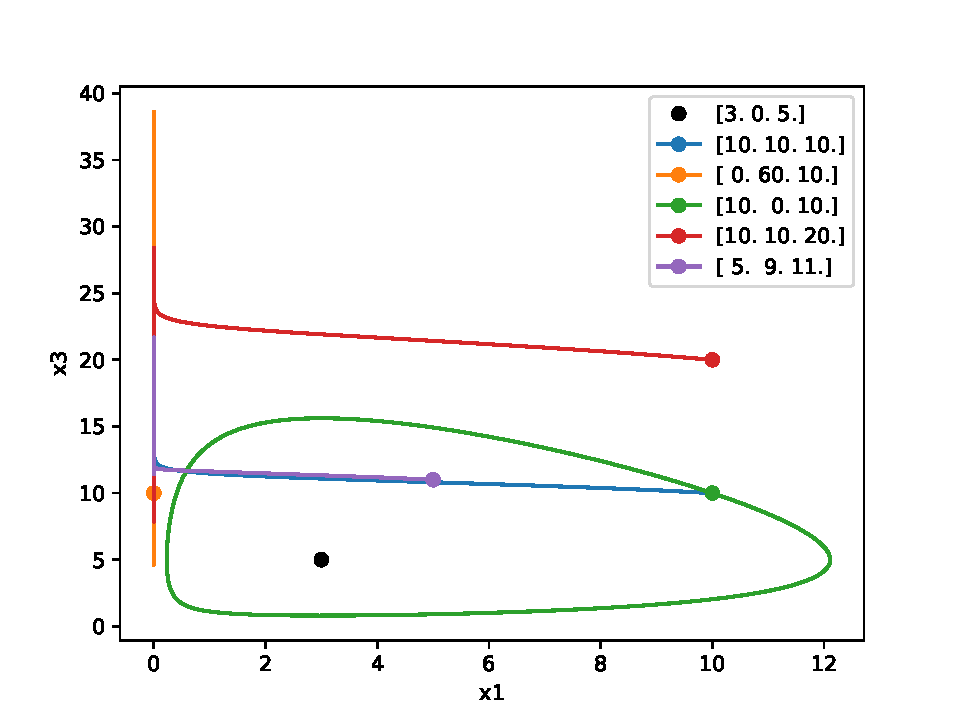
\includegraphics[width=8cm]{pictures/x_13phase.pdf}
        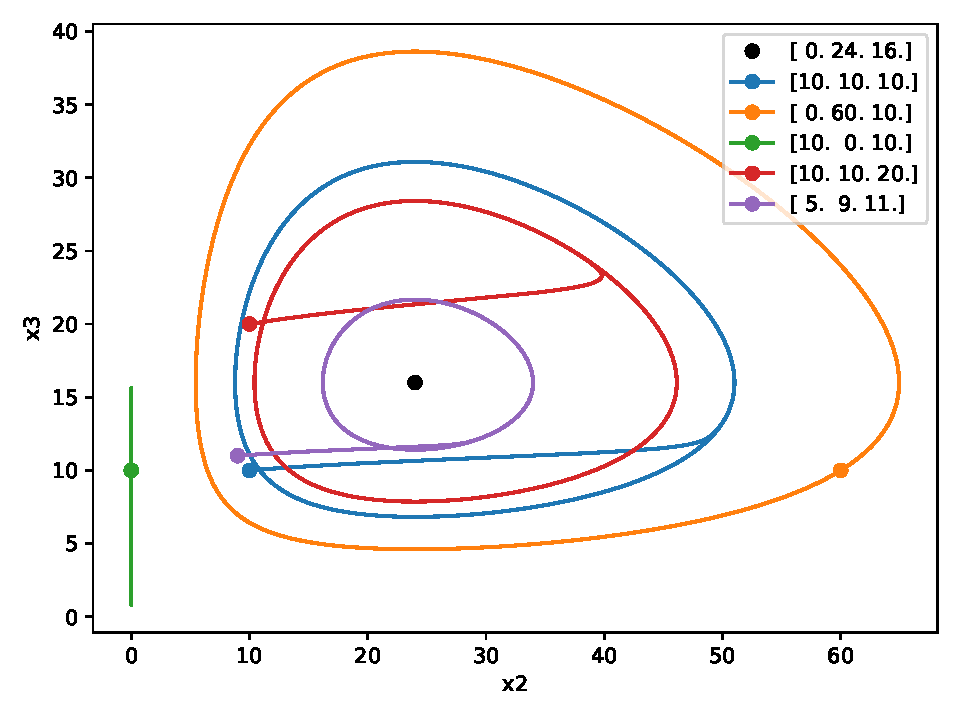
\includegraphics[width=8cm]{pictures/x_23phase.pdf}
        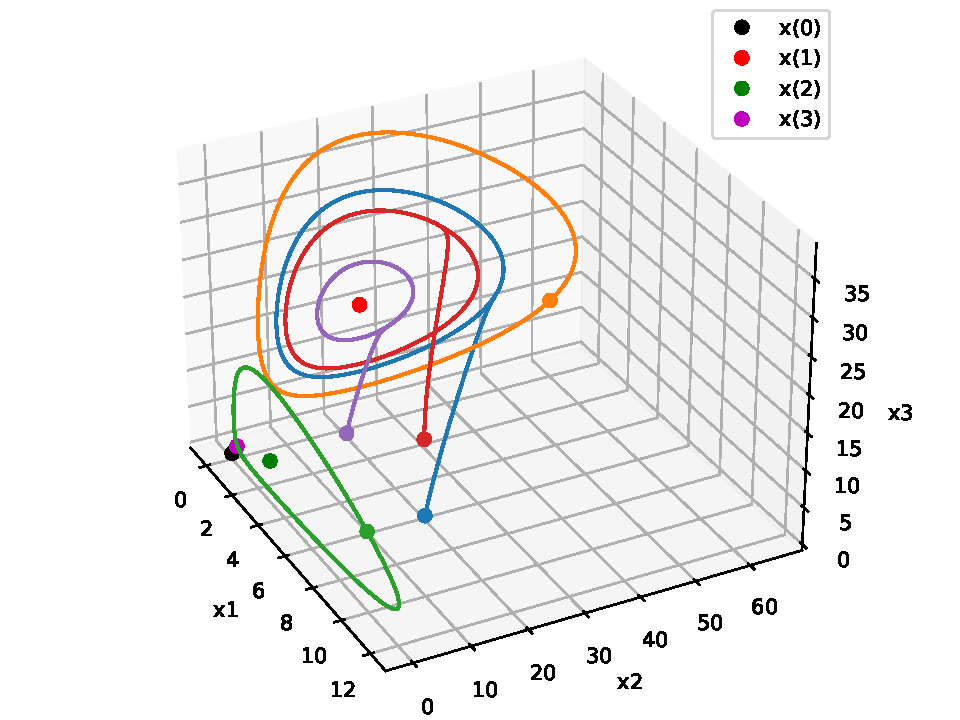
\includegraphics[width=8cm]{pictures/x_phase3.pdf}
        \caption{На отрезке времени \( [0, 3] \).} \label{lv3d}
    \end{figure}
    На рисунке \ref{lv3d} видно, что если присутствует вторая популяция хищников, то популяция жертв вымрет, а хищники останутся конкурировать друг с другом и никогда не вымрут. 
